\documentclass{article}
%\usepackage[a4paper, total={6in, 8in}]{geometry}
\usepackage{geometry}
\geometry{
a4paper,
total={210mm,297mm},
left=20mm,
right=20mm,
top=-2mm,
bottom=2mm,
}
%\usepackage[margin=0.5in]{geometry}

\usepackage{amsmath,amssymb}
\usepackage{ifpdf}
%\usepackage{cite}
\usepackage{array}
\usepackage{mdwmath}
\usepackage{pdfpages}
\usepackage{hyperref}
\usepackage{mdwtab}
\usepackage{arevmath}     % For math symbols
\usepackage{eqparbox}
\usepackage{algorithm}
\usepackage{algpseudocode} 
\usepackage{graphicx}
%\onecolumn
%\input{psfig}
\usepackage{color}
\usepackage{graphicx}
\setlength{\textheight}{23.5cm} \setlength{\topmargin}{-1.05cm}
\setlength{\textwidth}{6.5in} \setlength{\oddsidemargin}{-0.5cm}

\renewcommand{\baselinestretch}{1}
\pagenumbering{arabic}

\begin{document}
\textbf{
\begin{center}
{
    \large{School of Engineering and Applied Science (SEAS), Ahmedabad University}\vspace{5mm}
}
\end{center}
\begin{center}{
\large{BTech(ICT) Semester IV: Probability and Random Process (MAT202)\vspace{4mm}\newline Special Assignment-Final Report}
}
\end{center}
}
\begin{itemize}
\large
    \item \textbf{Group No. : SB - 4}
    \item \textbf{Group Members:\\ Harshil Mehta - AU1841010 \\ Raj Mehta - AU1841018 \\ Manav Patel - AU1841037}
    \item \textbf{Project Area : Biology}
    \item \textbf{Project Title : Disease Prediction and Analysis Of Schizophrenia}
\end{itemize}
\newpage 
\large{\section{Introduction}


\subsection{General discussion}
Schizophrenia is a chronic mental disorder. Many symptoms like Anger (Extreme), Mental confusion, Disorganised behaviour, unexpected memory loss leads to a disease named Schizophrenia. It's almost a non-curable disease. In some case it can improve conditions with help of happy environment, Psychotherapy and by some very expensive rehabilitation.On an average, only about 1\% of the total population is affected by this disease. Mostly it occurs due to psychosocial factors, problems during birth, malnutrition before birth and tragic(obsessive) events caused by the environmental factors faced by people.It can also cause Mental Hallucinations.}
\large
\subsection{General related work}

How will we view schizophrenia in 2030?[1] Schizophrenia today is a chronic, frequently disabling mental disorder that affects about one per cent of the world’s population.After a century of studying schizophrenia, the cause of the disorder still remains unknown.[2]Therefore there is an essential need for a probabilistic model which could quantify on the likeliness of a person having this disorder.[3]Also, there are theories and paperworks which empahsis on the complex modeling of schizophrenia but lack a basic inference - deriving model which could lead to better understanding.[4] The major modeling is done through Hardy - Weinberg Equilibrium.[5] Also, not much has been done in this field regarding probabilistic modeling and based on Inference deriving. \\ \\
Other related articles:
\begin{itemize}
    \item Bhattacharya, and Souvik. “Markov Chain Model to Explain the Dynamics of Human Depression.” \emph{Journal of Nonlinear Dynamics}, Hindawi, 18 Mar. 2014,\\ \url{www.hindawi.com/journals/jndy/2014/107164/}.
    \item Vivian-Griffiths, Timothy, et al. “Predictive Modeling of Schizophrenia from Genomic Data: Comparison of Polygenic Risk Score with Kernel Support Vector Machines Approach.” \emph{Wiley Online Library}, John Wiley and Sons, Ltd, 4 Dec. 2018, \url{www.onlinelibrary.wiley.com/doi/full/10.1002/ajmg.b.32705}.
    \item “US20150224120A1 - Compositions and Methods for Treating Hyperprolinemia-Associated Mental Disorders.” \emph{Google Patents}, Google,\\ \url{www.patents.google.com/patent/US20150224120A1/en}.
    \item Learning, Lumen. “Biology for Majors I.” \emph{Lumen}, \\ \url{www.courses.lumenlearning.com/wm-biology1/chapter/reading-penetrance-and-expressivity/}.
\end{itemize}

\newpage

\large
\subsection{Close related Work}

Main articles:
\begin{itemize}
    \item \textbf{Base article:}\\ \\
    Paek, Myung Jae, and Ung Gu Kang. “How Many Genes Are Involved in Schizophrenia? A Simple Simulation.” \emph{Progress in Neuro-Psychopharmacology and Biological Psychiatry}, Elsevier, 24 Apr. 2012, \url{www.sciencedirect.com/science/article/abs/pii/S0278584612000875}.
    \item “Allele Frequency \& the Gene Pool (Article).” \emph{Khan Academy}, Khan Academy,\\ \url{www.khanacademy.org/science/biology/her/heredity-and-genetics/a/allele-frequency-the-gene-pool}.
    \item Insel, Thomas R. “Rethinking Schizophrenia.” \emph{Nature News}, Nature Publishing Group, 10 Nov. 2010, \url{www.nature.com/articles/nature09552?page=7}.
\end{itemize}


\subsection{Motivation}
\large
The main motivation behind our current work is due to minimal quantitative work/analysis done in this subject.The Literature and Data analysis done by previous research has been based more upon Qualitative analysis of the disease . Higher algorithm like speech recognition, concepts of Deep - learning and Machine learning have been used to study cases and prepare data-sheets. So, our basic idea is to quantify schizophrenia and it's chances simple concepts of Probability and Random Process and basic mathematical modeling.

\large
\subsection{Problem Case Study}
Prediction of Schizophrenia is an uncertain problem. \\ \\
In our probabilistic model, one of the category which affects Schizophrenia i.e.  \textbf{Genes} is studied(and quantified). \\
Here some theories and concepts are applied to solve the uncertain problem. \\
There are different scenarios in which this is classified: \\ \\
Consider Total population as X. \\
Now Let XP be the patient population, so the remaining population will be  X - XP. \\
Now the cases that are to be calculated are quite obviuos for prediction of Schizophrenia in offspring: \\ \\
Mating Chances(Or Marriage Possibilities)
\begin{itemize}
    \item 1 person from XP and 1 person from (X - XP)
    \item both the person from XP.
    \item both the person from X - XP.(For more details refer algorithm Section) 
\end{itemize}
Theories used in this model: \\
\textbf{Hardy Weinberg Equilibrium, Strachan Hierarchy, Total Probability and Relative frequency Approach}.
\newpage 
In this work, the Hardy Weinberg Equilibrium and Joint Probability theory is applied along with the calculations of N and T using Total Probability Theorem. \\
Where N is number of Genes and T is pathogenic genes involved in Schizophrenia. \\
Strachan Hierarchy is used to plot bar chart and show comparison. \\
\\There are few assumptions of this theory: \\

\large{\textbf{Assumptions:}} \\ \\
\begin{itemize}
    \item Large population of Genes.
    \item No selection. (No biasing)
    \item No mutation. (No new genes can be produced from any combination of the two genes)
    \item Stable Allele Frequency.
    \item There are only two types of Genes involved. (For the sake of simplicity, just consider one of them as Dominant Gene and other as Recessive Gene)
\end{itemize}
\newpage
\large
\section{DATA ACQUISITION}
Yes, our special Assignment is Data Dependent. \\ \\
So, as we don't have any particular data sheets.As we don't have available data/statistics online.\\ We have generated random data-sets according to realistic figures given in :
\begin{itemize}
    \item Paek, Myung Jae, and Ung Gu Kang. “How Many Genes Are Involved in Schizophrenia? A Simple Simulation.” \emph{Progress in Neuro-Psychopharmacology and Biological Psychiatry}, Elsevier, 24 Apr. 2012, \url{www.sciencedirect.com/science/article/abs/pii/S0278584612000875}.
\end{itemize}
The random data generated is of no. of genes in a particular person with the dominance of its alleles'. \\
After generating this data set, we calculate the likeliness according to the formulas.

\newpage

\large
\section{Probabilistic Model Used/ PRP Concept Used}
\textbf{Probabilistic modelling}\\
Assumptions based on data: (are shown above)
\\
1) Total population of the world is approximately equal to 7 billion.
\\
2) Total schizophrenia patients in the world are approximately 1 \% of the total population.
\\
$\therefore$ Total patients = 7million,
\\
Now,
\\
Dividing the population into two part:\\ \\ 
\textbf{a)} Schizophrenic patients which constitutes the \textbf{Patient population} denoted as \textbf{PP}.
\\
\textbf{b)} Non - Schizophrenic patients which constitutes the \textbf{Non Patient population} denoted as \textbf{NP}.
\\
Now, Two odds of the offspring having Schizophrenia is determined by \textbf{Hardy Weinberg equilibrium} denoted as \textbf{HWE}\\
According to HWE, total probability of NP and PP is equal = 1.
\\
$\therefore$ \boxed{PP + NP = 1}
\\
Now, the genes of the offspring are the combinations of genes of both the parents.
\\
$\therefore$ squaring both sides we get
\begin{equation*}
    \boxed{PP^2 + 2\times PP\times NP + NP^2 = 1}
\end{equation*}
\\
As the schizophrenic allele is dominant compared to the non-schizophrenic allele. \\ \\$\therefore$ Probability of the offspring having schizophrenia is Prob(PP*PP) + Prob(2*NP*PP)
\\
and subtracting this from the total probability we get the probability of the offspring not having schizophrenia. which is Prob(2*NP*NP).
\\
Therefore,using the equations of \textbf{HWE} there are total 3 cases possible.
\\
\\
a) Offspring is the result of mating of two parents where both the parents belong to patient population (PP,PP). \\Here allele frequency of the dominant allele = 0.80 and allele frequency of recessive allele is 0.20
\\
\begin{figure}
    \centering
    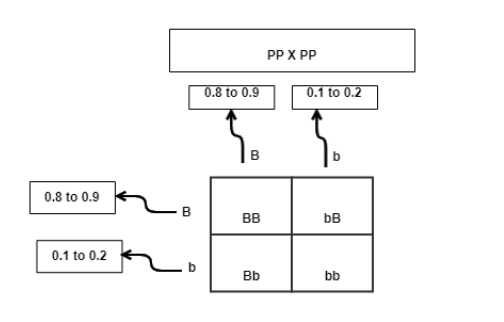
\includegraphics{PPXPP.PNG}
    
    \caption{case a): PP X PP}
\end{figure}
\\
\\
b) Offspring is the result of mating of two parents where both the parents belong to non patient population (NP,NP). \\Here allele frequency of the dominant allele = 0.99 and allele frequency of recessive allele is 0.01
\\
\begin{figure}
    \centering
    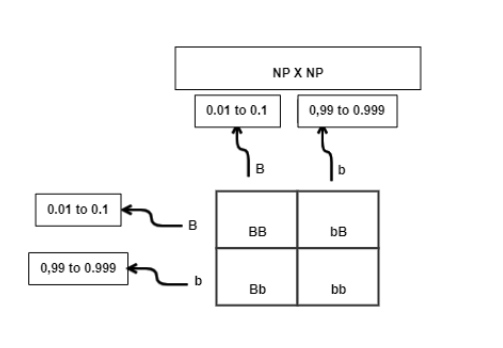
\includegraphics{NPXNP.PNG}
    
    \caption{case b): NP X NP}
\end{figure}
\\
\\
c)Offspring is the result of mating of two parents where one of the parent belong to non patient population(PP) and other one belong to (NP). \\Here allele frequency of the dominant allele = 0.99 and allele frequency of recessive allele is 0.01.
\\
\begin{figure}
    \centering
    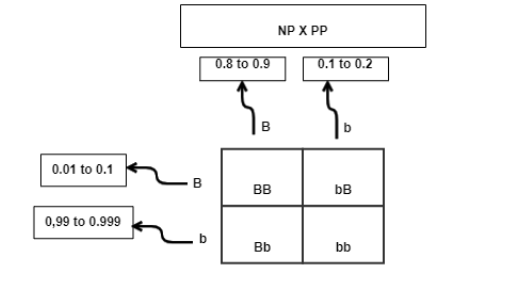
\includegraphics{NPXPP.PNG}
    \caption{case c): NP X PP}
\end{figure}

$\therefore$ In all three cases,
\begin{equation*}
    \text{Chances of Schizophrenia} = \text{Allele\_frequency}*(BB) + 2*\text{Allele\_frequency}*(Bb)
\end{equation*}
And
\begin{equation*}
    \text{Chances of the offspring of not having schizophrenia} = \text{Allele\_frequency}*(bb).
\end{equation*}
$\therefore$ Both these values are different for all three cases.
\newpage

\large
\section{Pseudo Code/ Algorithm}
\textbf{Pseudo Code}

\begin{algorithm}
\caption{Function For Obtaining Probability according Hardy-Weinberg Equilibrium }
\begin{algorithmic}[1]
\Function{Solve\_forN\_T}{frequency,ratio}  
    \State \Return{ratio$\times$(frequency * frequency + 2*(frequency)(1 - frequency))}          \Comment{Using HWE}
\EndFunction
\end{algorithmic}
\end{algorithm}


\begin{algorithm}
\caption{Function For Generating Random Data sets between input range}
\begin{algorithmic}[1]
\Function{GenerateRandomData}{ratio,startPoint,endPoint}
    \For{$i = 1,2$ $\ldots 100$}
        \State Random\_Value = Random($20,160$) \Comment{Uniform random data}
        \State Threshold\_Frequency.add(Random\_Value)
        \State Probability\_ans.add(Solve\_forN\_T(Random\_Value,ratio))
        \EndFor
\EndFunction
\end{algorithmic}
\end{algorithm}

\begin{algorithm}
\caption{Function For Solving Case-wise with inter Population mating}
\begin{algorithmic}[1]
\Function{solve\_probability\_case}{Allele\_A\_freq,Allele\_B\_freq}
    \State Offspring\_Probability = [(Allele\_A\_freq * (1 - Allele\_B\_freq)) + (Allele\_A\_freq * Allele\_B\_freq) + ((1 - Allele\_A\_freq)*(1 - Allele\_B\_freq))]
    \State \Return{Offspring\_Probability}  \Comment{Using Joint Probability Theorem}
\EndFunction
\end{algorithmic}
\end{algorithm}

We have also, used user defined functions and inbuilt functions for plotting different graphs and plots by programming.\\

\begin{algorithm}
\caption{Function For Strachan Hierarchy}
\begin{algorithmic}[1]
\Function{show\_Strachan\_hierarchy}{Probability}
    \State performance = [Probability, Probability*$0.92$, Probability*$0.74$,
                   Probability*$0.53$, Probability*$0.48$, Probability*$0.31$, Probability*$0.28$]
    \State plot performance[]
    \State \Return{performance}  \Comment{Hierarchy}
\EndFunction
\end{algorithmic}
\end{algorithm}

Next is the algorithm to obtain bar graph deduced from strachan's hierarchy.

\begin{algorithm}
\caption{Procedure For Solving each Probabilistic cases with inter Population mating}
\begin{algorithmic}[1]
\Procedure{main}{}
    \State GenerateRandomData($(0.01*0.01), 0.8, 0.99$)     \Comment{For case of PP vs PP}
    \State Rel\_Probability1 $\leftarrow$ solve\_probability\_case($0.8, 0.8$)
    \State GenerateRandomData($(0.99*0.99), 0.00001, 0.01$)    \Comment{For case of NP vs NP}
    \State Rel\_Probability2 $\leftarrow$ solve\_probability\_case($0.01, 0.01$)
    \State GenerateRandomData($(0.99*0.01$), random.uniform($0.001, 0.01$),random.uniform($0.8, 0.95$) \\    \Comment{For case of PP vs NP}
    \State Rel\_Probability3 $\leftarrow$ solve\_probability\_case($0.01, 0.8$)
\EndProcedure
\end{algorithmic}
\end{algorithm}

\newpage
\null\newpage

\section{Coding and Simulation}

\subsection{Simulation Framework}
    \hspace{7mm} \textbf{Assumptions:}
\begin{itemize}
    \item Total Population = 7 billion.
    \item Patient Population(Affected by Schizophrenia) = 1 \% of Total Population
    \item Non Patient Population = Total - Patient Population
    \item 3 mating cases of case studies. 
\end{itemize}
Now, The Number of genes($N$) are generated randomly between 20 and 160 according to the base article. \\
The allele frequency($T$) for the dominant gene is randomly generated between 0.8 to 0.95 and the allele frequency for the recessive gene is generated between 0.00001 to 0.01 according to the base article. \\ \\ 
Both Relative and Absolute Probabilities are calculated.  

\subsection{Reproduced Figures}

We have used MatlibPlot in Python to produce desired plots.

\includegraphics[scale=0.5]{fg1.PNG} \  \ \ \ \ \ \ \ \ \ \
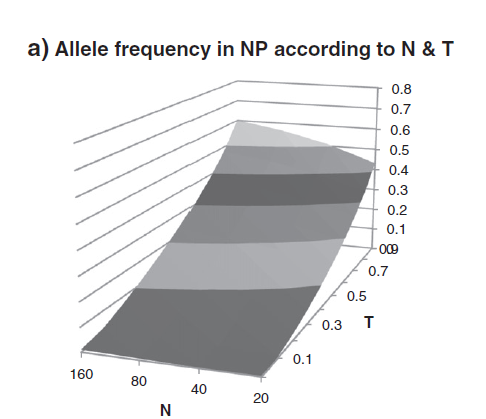
\includegraphics[scale=0.65]{article1.PNG} 
\newline
\\
\textbf{Allele frequency in NP according to N and T}
\newline
\\
\\
\\
\\
\\
\\
\\
\newline
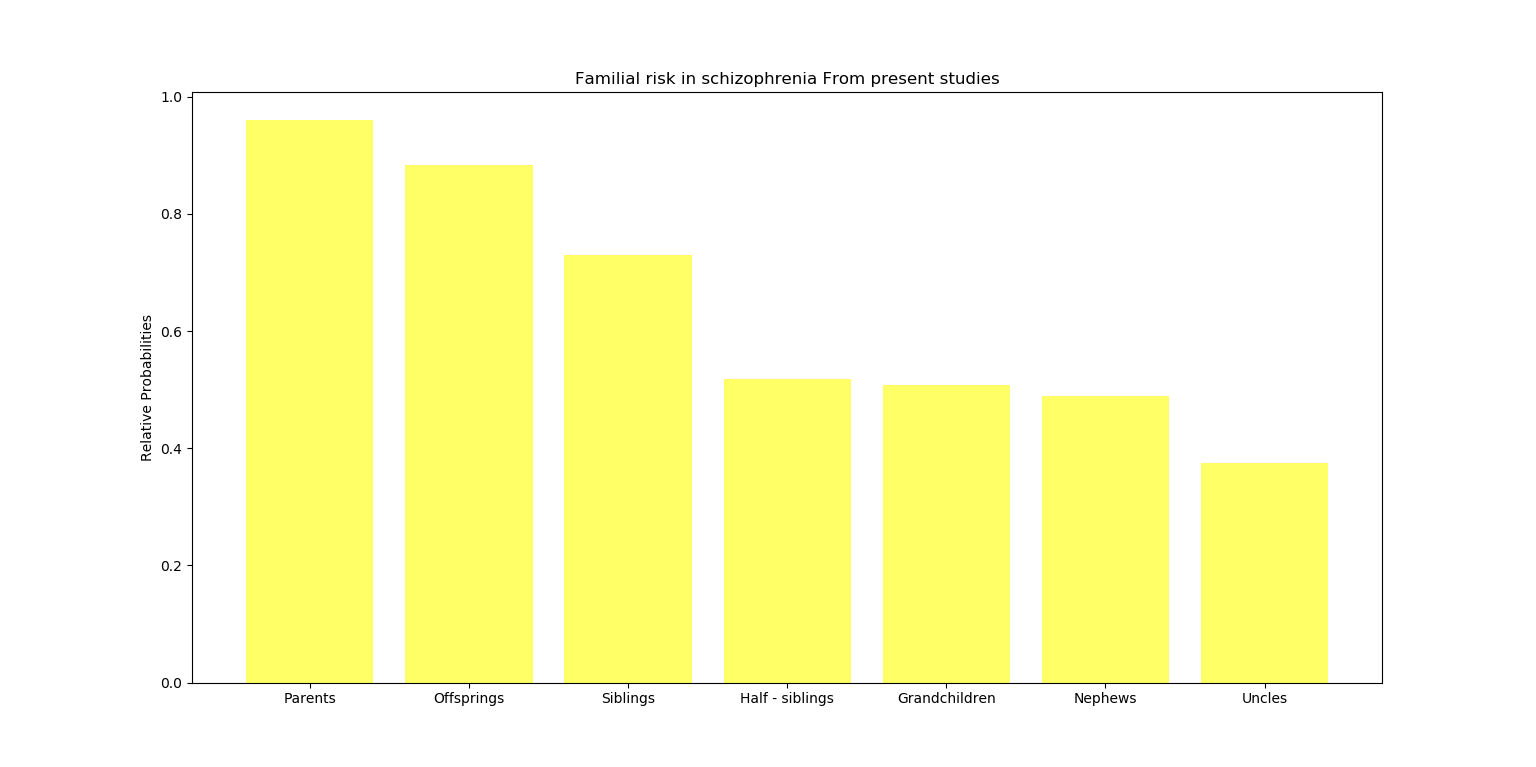
\includegraphics[scale=0.25]{Present_studies_OurWork.png}
\  
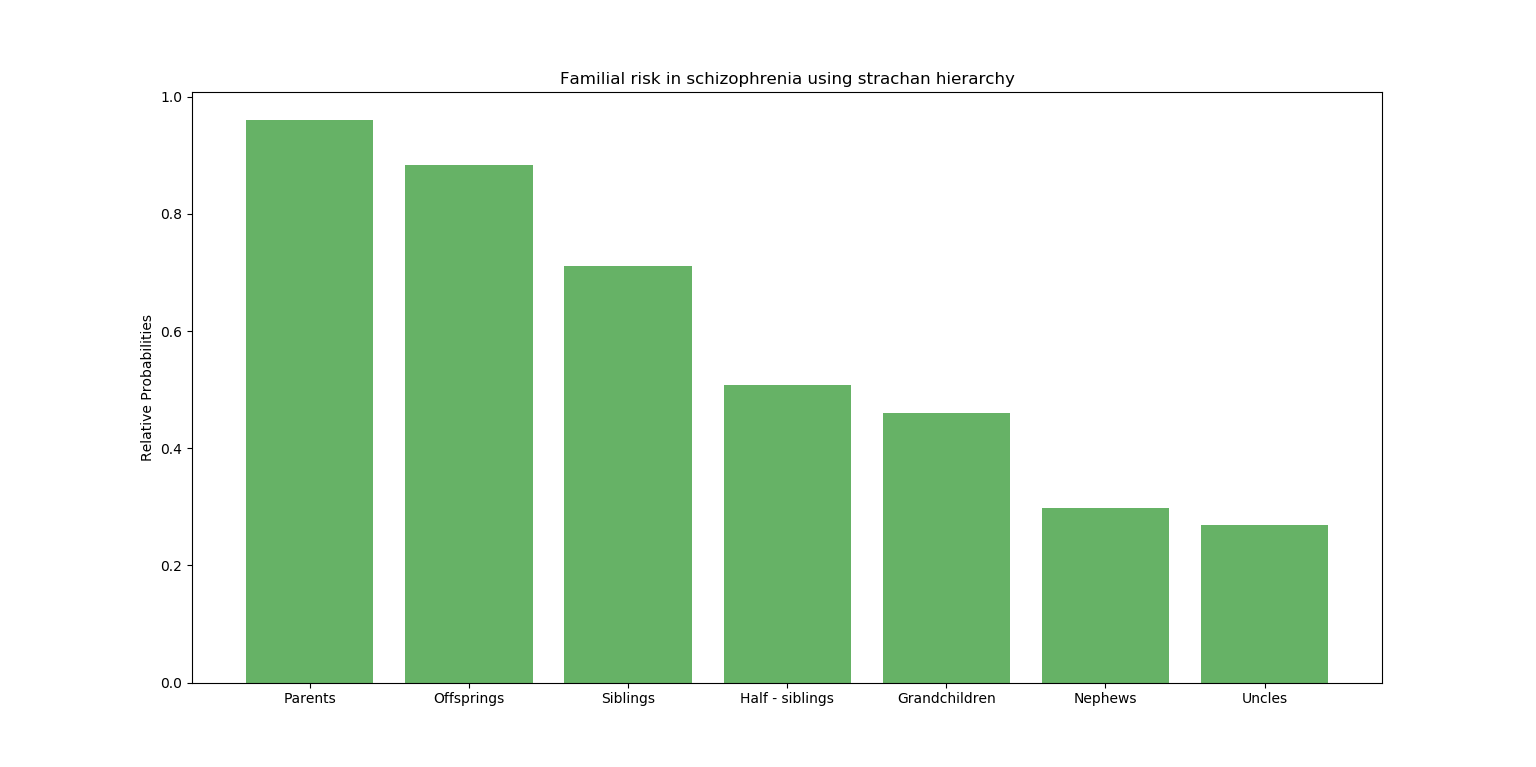
\includegraphics[scale=0.25]{Strachan-Hierarchy.png} 
\newline
\\
\textbf{Familial risk in Schizophrenia using present studies VS strachan hierarchy only for the case of PP vs PP}
\\
\\
\\
\\
\\
\\
\\
\newline
\newline
\includegraphics[scale=0.5]{fg2.PNG} \  \ \ \ \ \ \ \ \ \ \
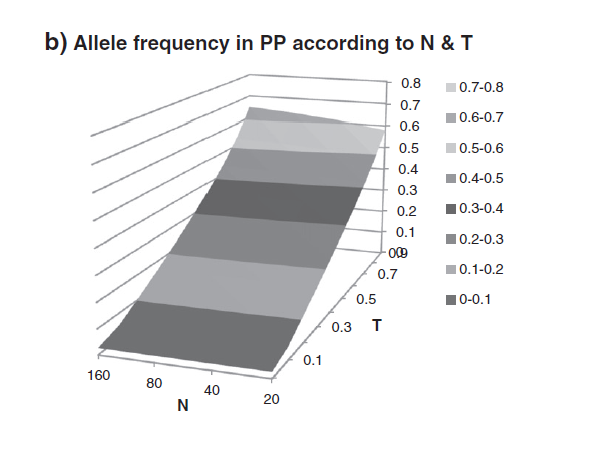
\includegraphics[scale=0.65]{article.PNG} 

\textbf{Allele frequency in PP according to N and T} \\ \\
\newpage
\section{Inference Analysis/ Comparison}

\textbf{Inference 1}:
\begin{itemize}
    \item As per the graphs and outputs obtained from the code, we can infer that as the with Increase in Number of genes and Allele Frequency $\xrightarrow{}$ Increase in Probability of having Schizophrenia.
    \item But, as the Allele is of dominant nature, increase in Allele Frequency is responsible for more increase in Probability than increase in Number of genes.
    \item Dependency of Probability is governed by: \\
    Number of genes($N$) $ << $ Allele Frequency($T$).
\end{itemize}
\textbf{Inference 2}:
\begin{itemize}
    \item As, we can observe from the Probability of each case, it is clear that by taking into account the Person from the Patient Population, the Probability of having Schizophrenia increases exponentially.
    \item Probability(PP vs PP) $ >> $ Probability(PP vs NP) $ >>> $ Probability(NP - NP).\\
    Here, PP denotes the person from patient Population and NP denotes the person from Non - Patient Population. 
\end{itemize}
\textbf{Inference 3}:
\begin{itemize}
    \item The Hierarchy which was prepared by Strachan in 1990 has shown relation between risk in families spread through Schizophrenia.
    \item Our studies has also shown very similar Hierarchy to Strachan's Hierarchy using bar graphs. 
\end{itemize}
Thus, from this inferences all of our study can be expressed in a more user - understandable language.\\
These thesis can help to analyze and quantify Schizophrenia in a more scrutinized manner.

\newpage
\section{Contribution of team members}

\subsection{Technical contribution of all team members} 
\begin{center}
 \begin{tabular}{||c|c|c|c||} 
 \hline
 Tasks & Harshil Mehta & Raj Mehta & Manav Patel \\ [0.5ex] 
 \hline\hline
 Task-1 & Coding(Part A) & Mathematical analysis & Resource/Info gathering \\ 
 \hline
 Task-2 & Simulation(bar charts) & Probabilistic Modeling & Coding(Part B) \\
 \hline
 Task-3 & Data-Correction & Testing & Inferencing \\
 \hline
 Task-4 & Inference-derivation & Simulation(graphs) & Case analysis \\ [1ex]
 \hline
\end{tabular}
\end{center}
\subsection{Non - Technical contribution of all team members} 
\begin{center}
 \begin{tabular}{||c|c|c|c||} 
 \hline
 Tasks & Harshil Mehta & Raj Mehta & Manav Patel \\ [0.5ex] 
 \hline\hline
 Task-1 & Introduction & Probabilistic Model Used & Problem/Case Study \\ 
 \hline
 Task-2 & Pseudocode/Algorithm & Simulation Framework & Data Acquisition \\
 \hline
 Task-3 & Inference analysis/Comparision & Reproduced Figures (Part1) & Reproduced Figures (Part2)\\ [1ex]
 \hline
\end{tabular}
\end{center}

\newpage 
\section{REFERENCES}

[1]. Marco Procopio(2005): \emph{Does god play dice with schizophrenia? A probabilistic model for the understanding of causation in mental illness}

[2]. Myung JaePaeka, Ung GuKangI(2012): \emph{How many genes are involved in schizophrenia?} A simple simulation

[3]. Ying Guo, DuBois Bowman and Clinton Kilts(2008:\emph{Predicting the Brain Response to Treatment Using a Bayesian Hierarchical Model With Application to a Study of Schizophrenia}

[4]. Elsevier Volume 127, Issues 1–3, April 2011, Pages 115-122 :\emph{Probabilistic learning and inference in schizophrenia}

[5].GENETIC EPIDEMIOLOGY , 05 June 2010: \emph{Impact of Hardy–Weinberg equilibrium deviation on allele-based risk effect of genetic association studies and meta-analysis}
\end{document}
